\documentclass[tikz,border=4pt]{standalone}
\usepackage{amsmath}
\begin{document}
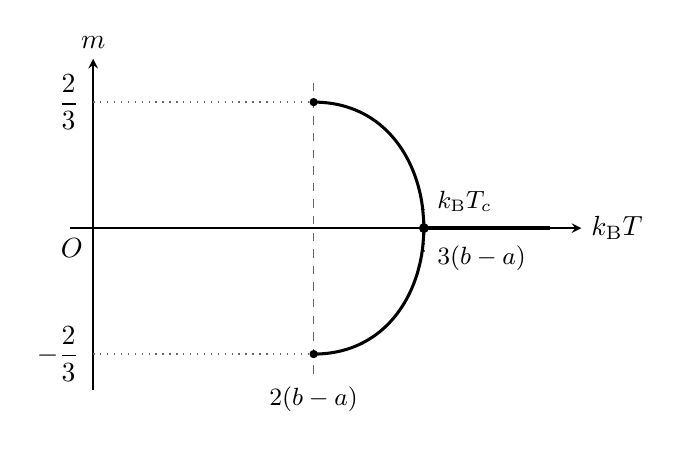
\begin{tikzpicture}[>=stealth, thick, scale=1.0]
  % Plot m(T) for k_B T > 2(b-a), using 4th-order Landau expansion:
  % m(T) = +/- (T/Tc) * sqrt(3*(1 - T/Tc)) for 2/3 < T/Tc < 1, and m = 0 for T >= Tc
  % Let x = 3.0 * (T/Tc) - 1.5 => T/Tc = 2/3 is x = 0.5; T/Tc = 1 is x = 1.5?
  % Better: let t = k_B T / (b-a), plot x = 1.4 * t (so t=2 -> x=2.8, t=3 -> x=4.2, t=4.2 -> x=5.88)
  % Vertical scale: y = 2.4 * m (so m = +/- 2/3 -> y = +/- 1.6)

  % Axes
  \draw[->, line width=0.55pt] (-0.3, 0) -- (6.2, 0) node[right] {$k_{\mathrm{B}}T$};
  \draw[->, line width=0.55pt] (0, -2.05) -- (0, 2.15) node[above] {$m$};
  \node[below left] at (0, 0) {$O$};

  % Vertical dashed reference lines at 2(b-a) and Tc = 3(b-a)
  \draw[dashed, line width=0.5pt, black!60] (2.8, -1.85) -- (2.8, 1.85);
  \draw[dotted, line width=0.5pt, black!60] (4.2, -0.3) -- (4.2, 0.3);
  \draw[dotted, line width=0.5pt, black!60] (0, 1.6) -- (2.8, 1.6);
  \draw[dotted, line width=0.5pt, black!60] (0, -1.6) -- (2.8, -1.6);

  % Upper branch m > 0 for t in [2, 3]
  \draw[line width=1.1pt]
    plot[domain=2.0:2.999, samples=100] ({1.4*\x}, {2.4*(\x/3)*sqrt(3 - \x)}) -- (4.2, 0);
  % Lower branch m < 0 for t in [2, 3]
  \draw[line width=1.1pt]
    plot[domain=2.0:2.999, samples=100] ({1.4*\x}, {-2.4*(\x/3)*sqrt(3 - \x)}) -- (4.2, 0);
  % High-T phase m = 0 for t >= 3
  \draw[line width=1.15pt] (4.2, 0) -- (5.8, 0);

  % Open/filled key points
  \fill (4.2, 0) circle (1.8pt);
  \fill (2.8, 1.6) circle (1.5pt);
  \fill (2.8, -1.6) circle (1.5pt);

  % Labels
  \node[left] at (-0.05, 1.6) {$\dfrac{2}{3}$};
  \node[left] at (-0.05, -1.6) {$-\dfrac{2}{3}$};
  \node[below, font=\small] at (2.8, -1.88) {$2(b - a)$};
  \node[below right, font=\small] at (4.24, -0.10) {$3(b - a)$};
  \node[above right, font=\small] at (4.24, 0.08) {$k_{\mathrm{B}}T_c$};
\end{tikzpicture}
\end{document}
